%\documentclass[border=5mm]{standalone}
%\usepackage{tikz}
%\usetikzlibrary{arrows.meta}
\begin{center}
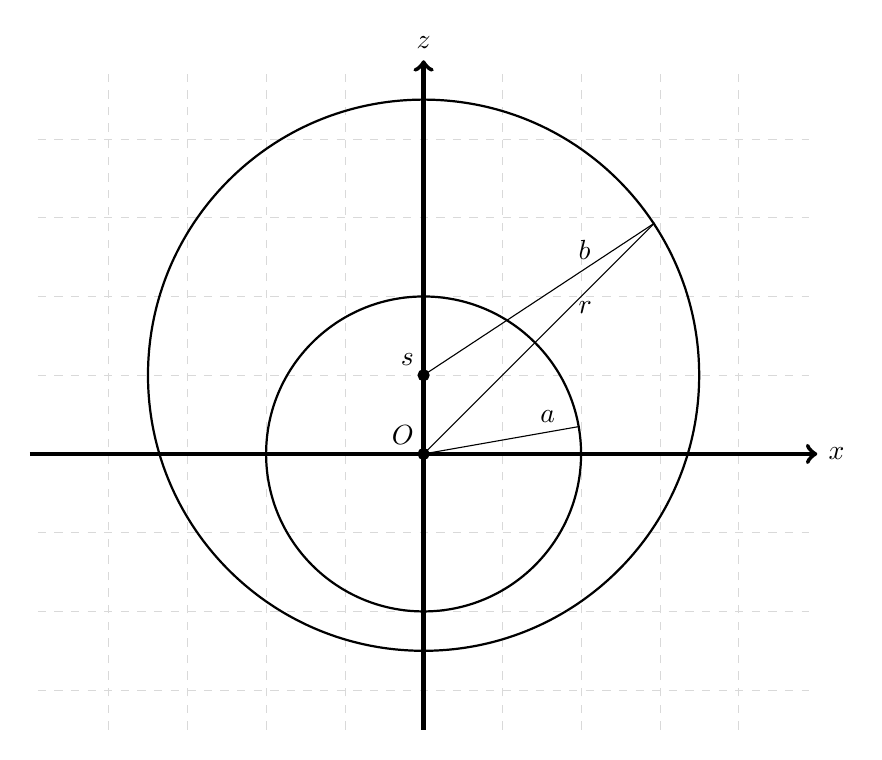
\begin{tikzpicture}

\draw[help lines, color=gray!30, dashed] (-4.9,-3.5) grid (4.9,4.9);
\draw[->,ultra thick] (-5,0)--(5,0) node[right]{$x$};
\draw[->,ultra thick] (0,-3.5)--(0,5) node[above]{$z$};

\draw [thick] circle [radius=2];
% \draw [thick] circle [radius=4];
% \draw (0,-1) circle (1.5cm);
\draw [thick] (0,1) circle [radius=3.5];

% \draw[double = gray!40, double distance=2cm, opacity=0.2] (0,0) circle (3);

\draw[-, rotate around={10:(0,0)}] (0,0) -- (2,0)  node [pos=0.8, above] {$a$};
\draw[-, rotate around={50:(0,1)}] (0,1) -- (3.35,0)  node[pos=0.7, above] {$b$};
\draw[-, rotate around={45:(0,0)}] (0,0) -- (4.15,0) node [pos=0.7, below] {$r$};
\draw[fill=black](0,0) circle (2 pt) node [anchor=south east] {$O$};
\draw[fill=black](0,1) circle (2 pt) node [anchor=south east] {$s$};

\end{tikzpicture}
\end{center}
